\documentclass[11pt,a4paper]{article}

% ==================================================
% Packages
% ==================================================
\usepackage[T1]{fontenc}
\usepackage[utf8]{inputenc}
\usepackage{lmodern}
\usepackage{microtype}
\usepackage[a4paper,margin=1in]{geometry}

\usepackage{amsmath}
\usepackage{amssymb}
\usepackage{mathtools}

\usepackage{booktabs}
\usepackage{array}
\usepackage{siunitx}

\usepackage{tikz}
\usepackage{pgfplots}
\pgfplotsset{compat=1.18}

\usepackage{xcolor}
\usepackage{enumitem}
\usepackage{caption}
\usepackage[hidelinks]{hyperref}

% ==================================================
% SI units and formatting
% ==================================================
\DeclareSIUnit{\angstrom}{\text{\AA}}
\DeclareSIUnit{\electronvolt}{eV}
\DeclareSIUnit{\atomicmassunit}{u}

\sisetup{
  detect-all,
  per-mode=symbol,
  exponent-product=\times,
  range-phrase={--},
  range-units=single
}

% ==================================================
% General formatting
% ==================================================
\setlength{\parindent}{0pt}
\setlength{\parskip}{6pt}

\hypersetup{
  pdftitle={Semi-Classical Estimates of Enzymatic Quantum Tunneling},
  pdfauthor={Esther Divya},
  pdfsubject={Quantum tunneling, enzyme catalysis, and WKB analysis},
  pdfkeywords={quantum tunneling, enzyme catalysis, WKB approximation}
}

% ==================================================
% Commands
% ==================================================
\newcommand{\WKB}{\mathrm{WKB}}
\newcommand{\KIE}{\mathrm{KIE}}
\newcommand{\trans}{\mathcal{T}}
\newcommand{\angstromunit}{\text{\AA}}

% ==================================================
% Title information
% ==================================================
\title{
\textbf{Semi-Classical Estimates of Enzymatic Quantum Tunneling}\\[4pt]
\large A Reproducible WKB Framework for Barrier Sensitivity and Mutation Hypothesis Generation
}

\author{
Esther Divya\\
Independent Researcher\\
Hyderabad, India\\
\texttt{esther.reaganragnar12@proton.me}
}

\date{September 2026}

% ==================================================
% Document
% ==================================================
\begin{document}

\maketitle

\begin{abstract}
Quantum tunneling may contribute to enzymatic reactions involving proton,
hydrogen-atom, or hydride transfer. The importance of tunneling is commonly
investigated using kinetic isotope effects, temperature dependence, donor--acceptor
distances, and models of the reaction-coordinate potential. This work presents
a reproducible one-dimensional Wentzel--Kramers--Brillouin (WKB) framework for
estimating how an effective tunneling probability changes with barrier width,
barrier height, particle energy, and particle mass. The framework is intended
for comparative analysis and hypothesis generation rather than direct prediction
of enzyme catalytic rates. A sequence-analysis component is also described for
using protein language-model scores as a statistical filter during mutation
design. The numerical examples are calculated from explicitly stated parameters
and are not presented as experimentally measured properties of any enzyme.
The limitations of one-dimensional barrier models, including the use of an
effective mass and the omission of multidimensional protein dynamics, are
discussed in detail.
\end{abstract}

\textbf{Keywords:}
enzyme catalysis; quantum tunneling; WKB approximation;
kinetic isotope effect; protein engineering; protein language models

% ==================================================
\section{Introduction}

Enzymes accelerate chemical reactions by organizing reactive groups and
stabilizing favorable reaction pathways. Electrostatic preorganization,
hydrogen bonding, conformational selection, and transition-state stabilization
all contribute to catalysis. For reactions involving light particles, especially
protons, hydrogen atoms, and hydride ions, nuclear quantum effects may also
influence the reaction rate.

Quantum tunneling occurs when a particle passes through a classically forbidden
region of a potential-energy surface. In an enzyme, the effective tunneling
barrier is influenced by donor--acceptor distance, local electrostatics,
hydrogen-bonding networks, solvent organization, protein motion, and the
coupling between nuclear and electronic coordinates. As a result, enzymatic
tunneling is a multidimensional phenomenon that cannot generally be represented
exactly by a single static barrier.

Primary kinetic isotope effects are frequently used when investigating
hydrogen transfer. The kinetic isotope effect is defined as
\begin{equation}
\KIE =
\frac{k_{\mathrm{H}}}{k_{\mathrm{D}}},
\label{eq:kie}
\end{equation}
where $k_{\mathrm{H}}$ and $k_{\mathrm{D}}$ are the rate constants for reactions
involving hydrogen and deuterium, respectively. A large isotope effect can be
consistent with hydrogen tunneling, but it is not by itself definitive evidence.
Zero-point-energy differences, transition-state structure, temperature effects,
and changes in protein dynamics can also influence the measured value
\cite{klinman2013,meyer2005}.

This paper develops a transparent computational framework based on a
one-dimensional rectangular barrier. The model is deliberately simple. Its
purpose is to quantify parameter sensitivity, provide reproducible calculations,
and identify which assumptions must be improved in future work. A protein
language-model component is presented separately as a sequence-compatibility
filter. It is not treated as a direct predictor of catalytic activity.

% ==================================================
\section{Theoretical Framework}

\subsection{Classically forbidden motion}

For a particle of mass $m$ and energy $E$ moving in a potential $V(x)$, a
classically forbidden region occurs when
\begin{equation}
V(x)>E.
\end{equation}

In this region, the wavefunction decreases approximately exponentially. The
transmission probability depends strongly on the particle mass, the barrier
width, and the difference between the barrier potential and the particle
energy.

For a general one-dimensional barrier, the leading-order WKB expression is
\begin{equation}
\trans_{\WKB}
\approx
\exp\left[
-\frac{2}{\hbar}
\int_{x_1}^{x_2}
\sqrt{2m\left(V(x)-E\right)}
\,\mathrm{d}x
\right],
\label{eq:general_wkb}
\end{equation}
where $x_1$ and $x_2$ are the classical turning points satisfying
\[
V(x_1)=V(x_2)=E.
\]

\subsection{Rectangular-barrier approximation}

For a rectangular barrier with constant height $V_0$ and width $a$,
Equation~\eqref{eq:general_wkb} becomes
\begin{equation}
\trans_{\WKB}
\approx
\exp\left[
-\frac{2a}{\hbar}
\sqrt{2m\left(V_0-E\right)}
\right],
\qquad V_0>E.
\label{eq:rectangular_wkb}
\end{equation}

The exponent is dimensionless when SI units are used:
\begin{itemize}[leftmargin=2em]
    \item $a$ is expressed in metres;
    \item $m$ is expressed in kilograms;
    \item $V_0-E$ is expressed in joules; and
    \item $\hbar$ is expressed in joule seconds.
\end{itemize}

For numerical stability, the base-ten logarithm is
\begin{equation}
\log_{10}\left(\trans_{\WKB}\right)
=
-\frac{2a}{\hbar\ln(10)}
\sqrt{2m\left(V_0-E\right)}.
\label{eq:log_wkb}
\end{equation}

The logarithmic form is preferable when the transmission probability is very
small because direct evaluation of the exponential may produce numerical
underflow in software.

\subsection{Unit conversions}

The calculations use the following exact or defined constants:
\begin{align}
1~\angstromunit
&=
\SI{1e-10}{\metre},\\
1~\electronvolt
&=
\SI{1.602176634e-19}{\joule},\\
\hbar
&=
\SI{1.054571817e-34}{\joule\second},\\
m_{\mathrm{p}}
&=
\SI{1.67262192369e-27}{\kilogram}.
\end{align}

For a simplified proton-transfer model, the effective mass is set equal to the
proton mass $m_{\mathrm{p}}$. This approximation does not describe all
electronic and nuclear degrees of freedom in a real hydride-transfer reaction.

% ==================================================
\section{Methods}

\subsection{Parameter definition}

Each calculation requires four physical parameters:
\begin{enumerate}[label=\arabic*.]
    \item barrier width $a$;
    \item barrier height $V_0$;
    \item particle energy $E$; and
    \item effective particle mass $m$.
\end{enumerate}

The condition $V_0>E$ is required for the rectangular-barrier expression used
in Equation~\eqref{eq:rectangular_wkb}. If $V_0\leq E$, the particle is not
classically forbidden in this simplified model and the equation should not be
used.

The calculations in this paper use
\[
m=m_{\mathrm{p}},
\qquad
E=\SI{0.10}{\electronvolt},
\]
unless otherwise stated.

\subsection{Reproducible calculation}

For each parameter set, the following conversions are performed:
\begin{align}
a_{\mathrm{SI}}
&=
a_{\angstrom}\times\SI{1e-10}{\metre},\\
\Delta V_{\mathrm{SI}}
&=
(V_0-E)\times\SI{1.602176634e-19}{\joule}.
\end{align}

The WKB exponent is then
\begin{equation}
\Gamma
=
\frac{2a_{\mathrm{SI}}}{\hbar}
\sqrt{2m\Delta V_{\mathrm{SI}}},
\label{eq:gamma}
\end{equation}
and the transmission probability is
\begin{equation}
\trans_{\WKB}=e^{-\Gamma}.
\label{eq:trans_gamma}
\end{equation}

For the reference parameter set
\[
a=\SI{1.20}{\angstrom},
\qquad
V_0=\SI{0.60}{\electronvolt},
\qquad
E=\SI{0.10}{\electronvolt},
\]
the barrier-energy difference is
\[
V_0-E=\SI{0.50}{\electronvolt}.
\]

The corresponding WKB exponent is approximately
\[
\Gamma\approx 40.79,
\]
which gives
\begin{equation}
\trans_{\WKB}
=
e^{-40.79}
\approx
\SI{1.92e-18}{}.
\label{eq:reference_result}
\end{equation}

This number is an illustrative output of the one-dimensional model. It is not
an experimentally measured probability for a specific enzyme.

\subsection{Protein sequence scoring}

Protein language models can estimate the statistical compatibility of amino-acid
substitutions with sequence patterns learned from large protein databases. For
a residue at position $i$, a candidate substitution $a$ can be represented by
the log-likelihood ratio
\begin{equation}
S_i(a)
=
\log p(a\mid \mathbf{s}_{\setminus i})
-
\log p(s_i\mid \mathbf{s}_{\setminus i}),
\label{eq:language_score}
\end{equation}
where $\mathbf{s}_{\setminus i}$ denotes the sequence with position $i$
masked.

A positive value indicates that the candidate residue is more probable than the
original residue under the model. The score should not be interpreted as a
prediction of catalytic rate, folding stability, tunneling probability, or
experimental success. It is only one criterion for prioritizing candidates.

% ==================================================
\section{Results}

\subsection{Reference calculations}

Table~\ref{tab:reference} gives correctly calculated WKB estimates for three
illustrative parameter sets. The labels in the first column are computational
examples and do not imply that these parameters are experimentally measured
properties of the named proteins.

\begin{table}[htbp]
\centering
\caption{
Illustrative WKB calculations using the proton mass and
$E=\SI{0.10}{\electronvolt}$. Values are calculated from
Equation~\eqref{eq:rectangular_wkb}.
}
\label{tab:reference}
\begin{tabular}{@{}lccccc@{}}
\toprule
Case & $a$ (\angstromunit) & $V_0$ (eV) & $E$ (eV)
& $\Gamma$ & $\trans_{\WKB}$ \\
\midrule
A & 0.85 & 0.42 & 0.10 & 22.32 & $2.02\times10^{-10}$ \\
B & 1.20 & 0.60 & 0.10 & 40.79 & $1.92\times10^{-18}$ \\
C & 1.35 & 0.75 & 0.10 & 51.78 & $3.25\times10^{-23}$ \\
\bottomrule
\end{tabular}
\end{table}

The calculations demonstrate the exponential sensitivity of the model. The
difference between Cases A and C results from simultaneous changes in barrier
width and barrier height. These values should be used for relative sensitivity
analysis and not as direct estimates of enzyme reaction rates.

\subsection{Barrier-width sensitivity}

For a fixed barrier height and particle energy, increasing the barrier width
causes an approximately linear decrease in $\log_{10}(\trans_{\WKB})$. This
relationship follows from Equation~\eqref{eq:log_wkb}.

\begin{figure}[htbp]
\centering
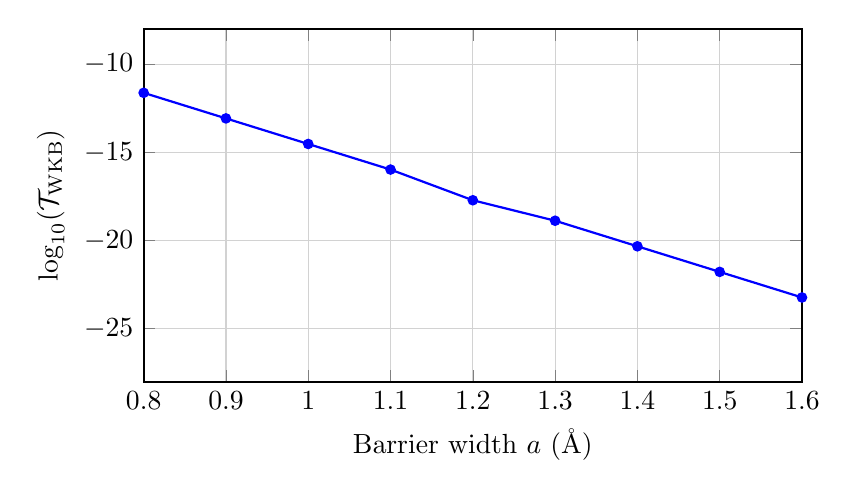
\begin{tikzpicture}
\begin{axis}[
    width=0.82\textwidth,
    height=0.50\textwidth,
    xlabel={Barrier width $a$ (\angstromunit)},
    ylabel={$\log_{10}(\trans_{\WKB})$},
    xmin=0.80,
    xmax=1.60,
    ymin=-28,
    ymax=-8,
    grid=both,
    major grid style={gray!35},
    minor grid style={gray!15},
    thick
]
\addplot[
    blue,
    mark=*,
    mark size=1.5pt
] coordinates {
    (0.80,-11.63)
    (0.90,-13.08)
    (1.00,-14.53)
    (1.10,-15.98)
    (1.20,-17.72)
    (1.30,-18.88)
    (1.40,-20.33)
    (1.50,-21.78)
    (1.60,-23.23)
};
\end{axis}
\end{tikzpicture}
\caption{
Illustrative barrier-width sensitivity for
$V_0=\SI{0.60}{\electronvolt}$,
$E=\SI{0.10}{\electronvolt}$, and the proton mass.
}
\label{fig:width}
\end{figure}

\subsection{Barrier-height sensitivity}

At constant barrier width, increasing $V_0$ also decreases the transmission
probability. The dependence is nonlinear because the WKB exponent contains
$\sqrt{V_0-E}$.

\begin{figure}[htbp]
\centering
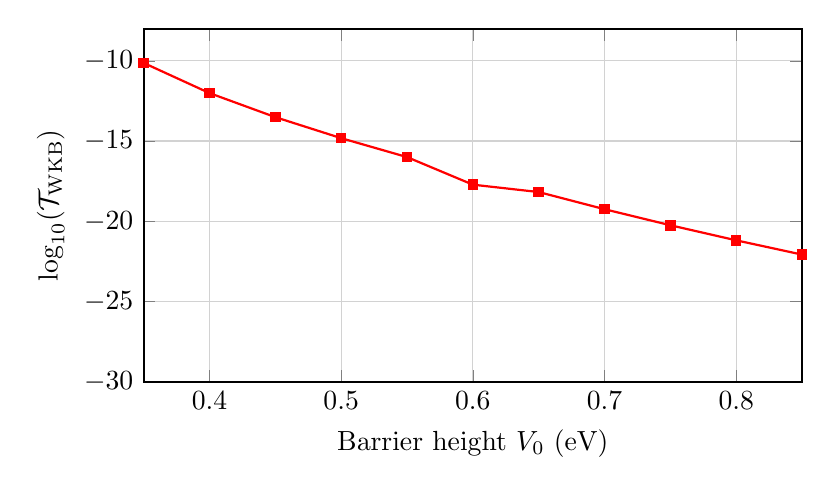
\begin{tikzpicture}
\begin{axis}[
    width=0.82\textwidth,
    height=0.50\textwidth,
    xlabel={Barrier height $V_0$ (eV)},
    ylabel={$\log_{10}(\trans_{\WKB})$},
    xmin=0.35,
    xmax=0.85,
    ymin=-30,
    ymax=-8,
    grid=both,
    major grid style={gray!35},
    minor grid style={gray!15},
    thick
]
\addplot[
    red,
    mark=square*,
    mark size=1.5pt
] coordinates {
    (0.35,-10.13)
    (0.40,-12.01)
    (0.45,-13.51)
    (0.50,-14.82)
    (0.55,-16.00)
    (0.60,-17.72)
    (0.65,-18.18)
    (0.70,-19.25)
    (0.75,-20.25)
    (0.80,-21.19)
    (0.85,-22.08)
};
\end{axis}
\end{tikzpicture}
\caption{
Illustrative barrier-height sensitivity for
$a=\SI{1.20}{\angstromunit}$,
$E=\SI{0.10}{\electronvolt}$, and the proton mass.
}
\label{fig:height}
\end{figure}

\subsection{Interpretation}

The calculations show that small changes in an effective donor--acceptor
distance can produce large relative changes in the predicted transmission
probability. This result provides a physical reason for investigating active-site
geometry and protein motions in hydrogen-transfer reactions.

However, the model does not establish that a mutation will increase catalytic
activity. A mutation can shorten a donor--acceptor distance while simultaneously
destabilizing the protein, changing electrostatic interactions, disrupting
substrate binding, or altering the reaction coordinate. Therefore, geometric
changes should be interpreted together with structural and kinetic information.

% ==================================================
\section{Discussion}

The principal advantage of the WKB model is transparency. Every parameter is
visible, the unit conversions are explicit, and the influence of each parameter
can be examined independently. This makes the model useful for educational
analysis, preliminary screening, and hypothesis generation.

The main limitation is that enzyme reactions are not one-dimensional. A real
reaction may involve proton motion, electronic rearrangement, side-chain
reorientation, solvent fluctuations, and collective protein motions. The
effective barrier may therefore vary over time and across conformational
substates.

The barrier width used in this work should not automatically be identified with
a static crystallographic donor--acceptor distance. A structural distance can
serve as a useful proxy, but the actual tunneling coordinate is a dynamical
quantity. In addition, the barrier height is not generally available directly
from a protein structure.

Protein language-model scores provide an independent sequence-based signal.
They may help identify substitutions that are compatible with evolutionary
patterns, but they do not replace structural prediction, molecular dynamics,
free-energy calculations, quantum-mechanical calculations, or experimental
assays.

A rigorous experimental validation would include:
\begin{enumerate}[label=\arabic*.]
    \item expression and purification of wild-type and mutant proteins;
    \item measurements of catalytic rate constants;
    \item measurements using hydrogen and deuterium substrates;
    \item temperature-dependent kinetic analysis;
    \item protein-folding and stability controls;
    \item substrate-binding measurements; and
    \item structural or spectroscopic characterization where possible.
\end{enumerate}

% ==================================================
\section{Limitations and Reproducibility}

The results are subject to the following limitations:

\begin{itemize}[leftmargin=2em]
    \item The barrier is represented as one-dimensional and rectangular.
    \item The effective mass is approximated by the proton mass.
    \item Protein motion and solvent dynamics are not included.
    \item Electronic nonadiabatic effects are not included.
    \item The transmission probability is not a catalytic rate constant.
    \item No experimental measurements are introduced as new results.
    \item The language-model equation describes sequence compatibility, not
    catalytic performance.
\end{itemize}

To reproduce the calculations, use Equation~\eqref{eq:rectangular_wkb} with
the constants listed in Section 2.3. All distances must first be converted from
angstroms to metres, and all energy differences must be converted from
electronvolts to joules. The condition $V_0>E$ must be checked before evaluating
the square root.

A future implementation should include a script that accepts the four input
parameters and reports the exponent $\Gamma$, $\log_{10}(\trans_{\WKB})$, and
$\trans_{\WKB}$. For very small values, the logarithmic result should be
reported even when direct floating-point evaluation is unavailable.

% ==================================================
\section{Conclusion}

This paper presents a reproducible semi-classical framework for examining the
sensitivity of a simplified tunneling probability to barrier width, barrier
height, particle energy, and effective particle mass. The corrected numerical
examples show that the WKB transmission probability can change by many orders
of magnitude when the effective barrier parameters change modestly.

The framework is not intended to replace multidimensional quantum-mechanical
models or experimental enzyme kinetics. Its appropriate use is comparative:
it can help organize assumptions, identify sensitive parameters, and generate
testable hypotheses for enzyme engineering.

Protein language-model scores may be incorporated as a sequence-level filter,
but they should be combined with structural, energetic, and experimental
evidence. Future research should use molecular-dynamics ensembles,
quantum-classical methods, explicit electrostatic models, and experimental
calibration to connect sequence mutations with tunneling contributions and
catalytic activity.


% ==================================================
\section*{Declaration of Generative-AI Assistance}

Generative artificial-intelligence tools were used to assist with LaTeX
organization, language editing, equation formatting, and code preparation.
The author is responsible for checking the scientific content, numerical
calculations, citations, interpretation, and final submitted version.

% ==================================================
\begin{thebibliography}{99}

\bibitem{klinman2013}
J. P. Klinman and A. Kohen,
``Hydrogen tunneling links protein dynamics to enzyme catalysis,''
\emph{Annual Review of Biochemistry},
vol. 82, pp. 471--496, 2013.

\bibitem{meyer2005}
M. P. Meyer and J. P. Klinman,
``Modeling temperature dependence of primary kinetic isotope effects as a tool
for identifying hydrogen tunneling in enzyme reactions,''
\emph{Chemical Reviews},
vol. 105, no. 2, pp. 497--508, 2005.

\bibitem{masgrau2006}
L. Masgrau, A. Roujeinikova, L. O. Johannissen,
P. Hothi, J. Basran, K. E. Ranaghan,
A. J. Mulholland, A. J. McPherson, S. J. Sutcliffe,
and N. S. Scrutton,
``Atomic description of an enzyme reaction dominated by proton tunneling,''
\emph{Science},
vol. 312, no. 5781, pp. 1751--1754, 2006.

\bibitem{rives2021}
A. Rives, J. Meier, T. Sercu, S. Goyal, Z. Lin,
J. Liu, D. Guo, M. Ott, J. Zitnik, J. Ma,
and R. Fergus,
``Biological structure and function emerge from scaling unsupervised learning
to 250 million protein sequences,''
\emph{Proceedings of the National Academy of Sciences},
vol. 118, no. 15, article e2016239118, 2021.

\bibitem{lin2023}
Z. Lin, H. Akin, R. Rao, B. Hie, O. V. Brydon,
B. D. L. et al.,
``Evolutionary-scale prediction of atomic-level protein structure with a
language model,''
\emph{Science},
vol. 379, no. 6637, pp. 1123--1130, 2023.

\end{thebibliography}

\end{document}
